\documentclass{beamer}
\usetheme{Warsaw}
\useinnertheme{umbcboxes}

\title{Representing Reactivity}
\subtitle{Compiling Resumptions for Handling, Signaling, and Semaphores}

\author{Benjamin Schulz}

%%%%

\usepackage{amsmath}
\usepackage{proof}

\newcommand{\forget}[1]{}
\newcommand{\qs}[0]{\ \ \ \ }

%%%%

\begin{document}

\maketitle{}

%%%% slide
\begin{frame}{What's to Talk About}

\begin{itemize}

\item{What a reactive resumption is and is not}

\item{Representing reactive control flow in RSI: New constructs}

\item{Reification of signaling in terms of control flow}

\item{Challenges, and lingering issues}

\end{itemize}

\end{frame}

%%%% slide
\begin{frame}{Recap: the Reactive Resumption Monad}

\begin{structure}{Resumptions, and Then Some}
\begin{onlinebox}{11cm}

$ReactT\ q\ r\ m\ a\ = D\ a\ |\ P(q, r \rightarrow m\ (ReactT\ q\ r\ m\ a))$\\

\begin{tabular}[t]{lll}
\\
$\eta\ v$ &$=$& $D\ v$\\
$(D\ v)\ \bigstar_{Re}\ f$ &$=$& $f\ v$\\
$(P\ (q,\ r))\ \bigstar_{Re}\ f$ &$=$& $P\ (q,\ \lambda p .\ (r\ p)\ \bigstar_m\ \lambda m .\ \eta_m\ (m\ \bigstar_{Re}\ f))$\\

\end{tabular}

\end{onlinebox}
\end{structure}

\medskip

\begin{itemize}

\item{$Re$ has the same basic control flow structure as $R$}

\item{In contrast to $R$, however, the body of an $Re$ term must be supplied with a response before resuming execution}

\item{Hence, the need for a $handler$, which is really an atom-wise, layer-specific projection:}

\end{itemize}

\begin{onlinebox}{10cm}

$handle\ ::\ Re\ a \rightarrow m\ (Re\ a)$\\
$\pi_{Re}\ r\ = handle\ r\ \bigstar_m\ \lambda r\prime .\ \pi_{Re}\ r\prime$\\

\end{onlinebox}

\smallskip

\emph{The definition of  the handler determines the global semantics}

\end{frame}

%%%% slide
\begin{frame}{Compiling Resumptions: Revised and Updated Strategy}

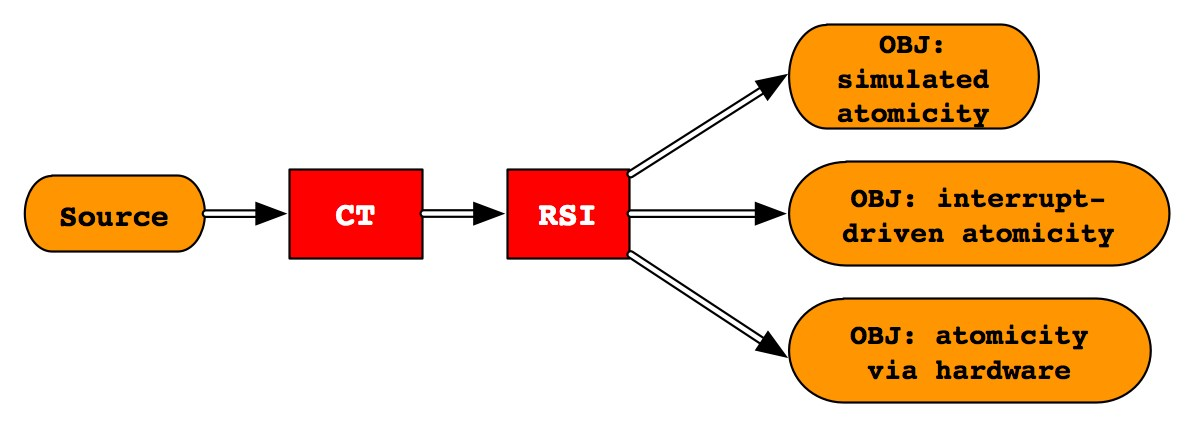
\includegraphics[width=9cm]{targets.jpg}

\begin{structure}{In a Nutshell}
\begin{itemize}
\begin{scriptsize}
\item{Use intermediate phase to compile imperative code, which is straightforward}

\item{Make resumptive/reactive control structures explicit}

\item{Use latter phases, i.e. backends, to compile control flow, which is highly implementation-dependent}

\item{All this makes it much easier to hit multiple targets}
\end{scriptsize}
\end{itemize}
\end{structure}

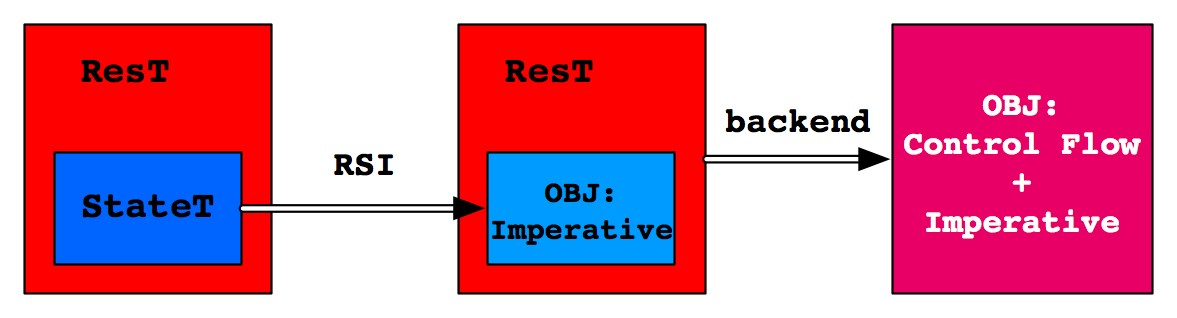
\includegraphics[width=9cm]{layers.jpg}


\end{frame}



%%%% slide
\begin{frame}{Reifying Re: Control Structures for Reactivity}

\begin{structure}{RSI Execution Stream Grammar}

\begin{tabular}[t]{llll}

\begin{minipage}[t]{4cm}

\begin{tabular}[t]{lll}
A &::=& L: \texttt{atom} \{ K \}\\
&$|$& L: \color{red}{\texttt{throw} \{ K \}}\\
\\
C &::=& A; C\\
&$|$& \texttt{bz} X C C C\\
\end{tabular}
\end{minipage}
&
\begin{minipage}[t]{3.5cm}
\begin{tabular}[t]{lll}

&$|$& \texttt{loop} C C\\
&$|$& \texttt{break} X\\
&$|$& \texttt{swr} R C\\
&$|$& \color{red}{\texttt{swt} R C}\\
\end{tabular}
\end{minipage}
&
\begin{minipage}[t]{3.75cm}
\begin{tabular}[t]{lll}

&$|$& \color{red}{\texttt{catch} R C}\\
&$|$& \texttt{jmp} R C\\
&$|$& \texttt{done}\\
\end{tabular}
\end{minipage}

\end{tabular}
\end{structure}

\begin{structure}{What's New}
\begin{itemize}

\item{\texttt{throw} produces an atomic action always followed by return of control to the caller}

\item{\texttt{catch} resumes execution with the response from the caller bound to the first argument}

\item{\texttt{swt} behaves exactly as \texttt{swr} (i.e. $resume_R$), but masks occurrences of \texttt{throw}}

\end{itemize}
\end{structure}

\end{frame}

%%%% slide
\begin{frame}{Basics: Reactive Atomicity}

\begin{structure}{Semantics of Reactive Step}

\begin{onlinebox}{8cm}

$step_{Re}\ ::\ m\ a\ \rightarrow Re\ a$\\
$step_{Re}\ \phi = P\ (Cont,\ \lambda Ack .\ \phi\ \bigstar_m\ (\eta_m \circ \eta_{Re}))$\\

\end{onlinebox}

\end{structure}

\bigskip

\begin{structure}{Compilation: an Operational Two-Step}
\begin{onlinebox}{9cm}

\begin{tabular}[t]{ll}
$\lceil step\ \phi \rceil_{Re} =$ &\texttt{throw \{ clr r\_req \};}\\
&\texttt{atom}\{ $\lceil \phi \rceil_K$ \texttt{; r\_nxt := L \};}\\
&\texttt{L: nop} \\

\end{tabular}

\end{onlinebox}

\medskip

\begin{itemize}

\item{The code in a reactive action is atomic, but it must be run in two steps}
\begin{itemize}\item{One to signal the handler}\item{Another to actually run the code once the OK is given}\end{itemize}

\item{In accordance with the reactive semantics and CT conventions, \emph{this will never run without application of a handler}, hence the need to communicate with the caller through \texttt{throw}}

%\item{In the conventional definition of $step_{Re}$, null signals are exchanged; hence clearing of the request register \texttt{r\_req}}

\end{itemize}
\end{structure}

\end{frame}

%%%% slide
\begin{frame}{Basics: Reactive Signaling}

\begin{structure}{Semantics of Reactive Signal}

\begin{onlinebox}{7cm}

$signal\ ::\ Req\ \rightarrow Re\ a$\\
$signal\ q = P\ (q,\ \eta_m \circ \eta_{Re})$\\

\end{onlinebox}

\end{structure}

\bigskip

\begin{structure}{Compilation: Throwing a Signal}
\begin{onlinebox}{9cm}

\begin{tabular}[t]{ll}
$\lceil signal\ q \rceil_{Re} =$ &\texttt{throw \{ $\lceil q \rceil_{Id}$ \};}\\
&\texttt{atom}\{\texttt{ r\_nxt := L \};}\\
&\texttt{L: nop} \\

\end{tabular}

\end{onlinebox}

\begin{itemize}

\item{Again, execution proceeds in two steps: one to signal, a second to run the next slice of code}

\item{Since $signal$ simply returns in $m$, the accompanying action simply returns the location of the next signal-atom pair}

\end{itemize}

\end{structure}


\end{frame}

%%%% slide

\begin{frame}{Next Steps: Reactive Sequencing}

\begin{structure}{Compilation: Putting \texttt{catch} to Use}
\begin{onlinebox}{11cm}

\begin{tabular}[t]{lll}

$\lceil signal\ q\ \bigstar_{Re}\ \lambda x .\  r \rceil_{Re}$ &=&\texttt{throw } \{$\lceil q\rceil_{Id}$\}; \texttt{catch x} $\lceil r \rceil_{Re}$\\
\\
$\lceil r\ \bigstar_{Re}\ \lambda x .\ r\prime \rceil_{Re}$ &=& $retsave\ x\ \lceil r \rceil_{Re}$; $\lceil r\prime \rceil_{Re}$\\

\end{tabular}

\end{onlinebox}
\end{structure}

\begin{itemize}

\item{Here, \texttt{catch} is used to encapsulate the binding of the response from the caller}

\item{Encapsulating the response-binding is important; otherwise, the caller might inadvertantly clobber it}

\item{In the general case, $retsave$ handles return-passing by making \texttt{x := r\_ret} the final statement in the preceding action}

\end{itemize}

\end{frame}

%%%% slide
\begin{frame}{Things Get Interesting: Reading Out Signals}

Handling i.e. running reactive resumptions requires deconstructing not just the underlying action, but also the request:

\begin{center}
\begin{onlinebox}{7cm}

$getreq\ ::\ Re\ a\ \rightarrow Req$\\
$getreq\ (P\ (q,\ \_)) = q$\\

\end{onlinebox}
\end{center}

\begin{structure}{Compiling Signal Read-Out}
\begin{onlinebox}{9cm}

$\lceil getreq\ r \rceil_{Re} =$ \texttt{swr} $eval \lceil r \rceil_{Re}$\\

\end{onlinebox}
\end{structure}

\begin{itemize}

\item{\texttt{swr} runs exactly one atomic action of the argument}

\item{Since all reactive actions produce two actions, one \texttt{throw} and one \texttt{atom}, only the request assignment in $\lceil r \rceil_{Re}$ will occur}

\end{itemize}

\pause

\begin{structure}{Compiling Signal Read-Out: Alternate}
\begin{onlinebox}{9cm}

$\lceil getreq\ r \rceil_{Re} =$ \texttt{\color{red}{getreq}} $eval \lceil r \rceil_{Re}$\\

\end{onlinebox}
\end{structure}

\smallskip

... alternatively, we could simply transcribe $getreq$, and push the details down the backend

\end{frame}

%%%% slide
\begin{frame}{Meat of the Matter: Reactive Context Switch}

\begin{structure}{Reactive \texttt{resume}}

\begin{onlinebox}{10cm}

\flushleft{$resume_{Re} ::\ Re\ a\ \rightarrow Rsp \rightarrow R\ (Re\ a)$}\\

\begin{tabular}[t]{lll}
$resume_{Re}\ r\ p\ = $&$case\ r\ of$\\
&$\ \ (P\ (\_,\ x))\ $&$\mapsto step_R\ (x\ p)$\\
&$\ \ (D\ v)\ $&$\mapsto step_R\ ((\eta_m \circ \eta_{Re})\ v)$\\

\end{tabular}

\end{onlinebox}
\end{structure}

\medskip

\begin{structure}{Compiling Reactive \texttt{resume}}

\begin{onlinebox}{11cm}

$\lceil resume_{Re}\ r\ p\rceil_{Re} =$ \texttt{atom\{r\_rsp := $\lceil p \rceil_{Id}$\}; swt} $eval(\lceil r \rceil_{Re})$\\

\end{onlinebox}

\end{structure}

\begin{itemize}

\item{The response to $r$ is passed through \texttt{r\_rsp}}

\item{\texttt{swt} runs the next action in $r$, ignoring the initial \texttt{throw}}

\item{The handler is assumed to be responsible for specifying the response to pass to $r$}

\item{This response is presumed to be determined, implicitly or explicitly, somewhere within the calling term}


\end{itemize}

\end{frame}

%%%% slide
\begin{frame}{An example: Simple Semaphores for a Shared Variable}

\begin{scriptsize}

\begin{tabular}[t]{ll}

main =\\
\qs\qs loop\_R\\
\qs\qs($\lambda$ r $\rightarrow$\\
\qs\qs\qs           getreq (fst r) $>>$= $\lambda$ q $\rightarrow$\\
\qs\qs\qs           step\_R (get Sem) $>>$= $\lambda$ ok $\rightarrow$\\
\qs\qs\qs            if (q == Grab) \&\& ok\\
           \\
\qs\qs\qs            then\\
\qs\qs\qs\qs             step\_R (put Sem False) $>>$\\
\qs\qs\qs\qs             resume\_Re (fst r) Grant $>>$= $\lambda$ t $\rightarrow$\\
\qs\qs\qs\qs             return (snd r, t)\\
\\
\qs\qs\qs           else\\
\qs\qs\qs\qs             if (q == Release)\\
\qs\qs\qs\qs\qs             then step\_R (put Sem True) $>>$ return (snd r, fst r)\\
\qs\qs\qs\qs             else \\
\qs\qs\qs\qs               resume\_Re (fst r) Deny $>>= \lambda$ t $\rightarrow$ return (snd r, t)\\
\qs \qs        ) \\

\end{tabular}
\end{scriptsize}

\begin{onlinebox}{11cm}

\begin{scriptsize}
\begin{itemize}
\item{$main$ acts as a handler that alternately locks and unlocks a shared variable $G$ in response to requests from two reactive streams}

\item{$main$ thus separates the two streams from direct access to the semaphore; only $Grant$ or $Deny$ responses control access to $G$}

\end{itemize}
\end{scriptsize}

\end{onlinebox}

\end{frame}

%%%% slide
\begin{frame}{Summary}

\begin{itemize}

\item{Reactive actions have two distinct components}
\begin{itemize}{\item{a signal}\item{an imperative action}}\end{itemize}

\item{These actions are compiled into paired \texttt{throw}-\texttt{atom} blocks}

\item{Reactive execution is reified in terms of \texttt{throw} and \texttt{catch}}

\item{Handling is reified in terms of \texttt{swr} and \texttt{swt}}

\item{Reactive signal deconstruction is tricky but possible, and may be handled either in terms of atomic execution or direct access to the stored program}

\item{Current compiler now produces working code for the semaphore example!}

\end{itemize}

\end{frame}

\begin{frame}{Thanks!}

\begin{structure}{Questions?}


\includegraphics[width=9cm]{questions}

\end{structure}

\end{frame}

\end{document}